\section{Gradient and Edge Following Integration}
\begin{frame}
	\frametitle{Edge Following}
		\textbf{Objective:} Algorithm to form  gradient  with  respect  to  reference  robot  first  and then bring the farthest robot near the reference robot by using edge following algorithm.  We are integrating the gradient formation and edge following experiments performed earlier.
\end{frame}

\begin{frame}
\frametitle{Flowchart}
\begin{figure}[H]
	\centering
	\fbox{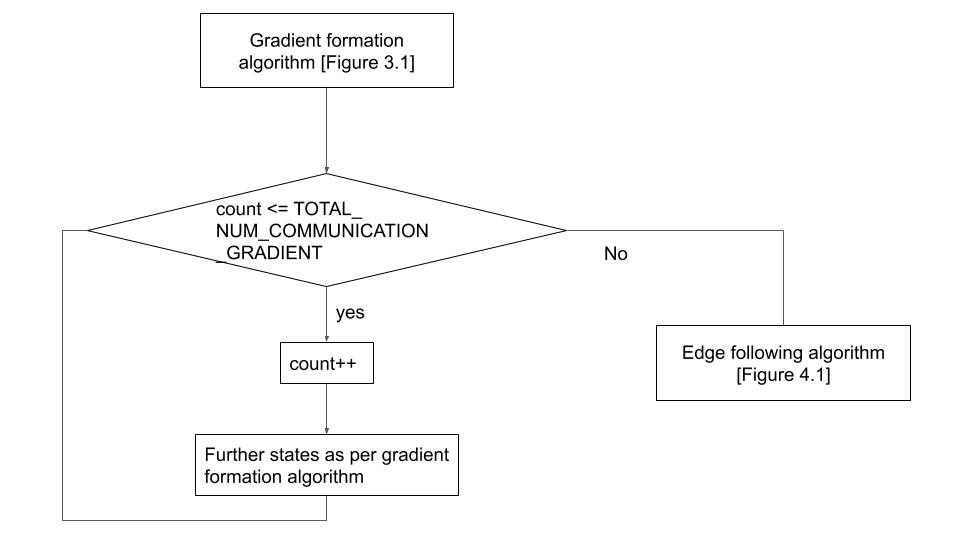
\includegraphics[scale=0.31]{images/flowchart-gradient&edge-following.jpg}}
	\caption{Integration of gradient formation and Edge following}
	\label{fig:Flowchart for integration of gradient formation and Edge following}
\end{figure}
\end{frame}

\begin{frame}
\frametitle{Demonstration}
\begin{figure}[H]
	\centering
	\fbox{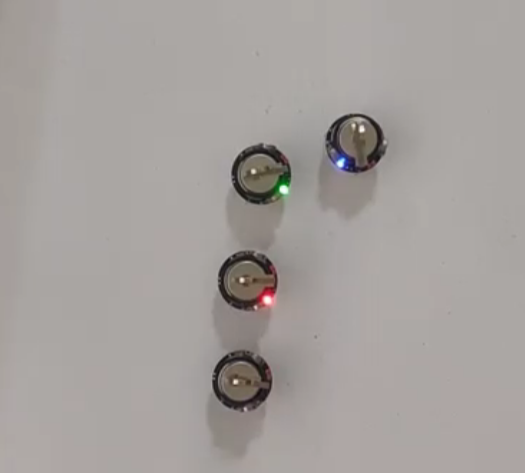
\includegraphics[width=2.4in]{images/gradient-edgefollowing.png}}
	\caption{\href{https://drive.google.com/file/d/1hssXnUnJvkTeVwVcXkR3x3gSFJD0FXtD/view}{Gradient formation and Edge following integration with \textit{TOTAL\_NUM\_COMMUNICATION\_GRADIENT=20} and \textit{TOTAL\_NUM\_COMMUNICATION = 15}}}
	\label{fig:Gradient formation and Edge following integration}
\end{figure}
\end{frame}


